\section{Leitner's learning box reviewed}

\emph{Leitner's learning box}\footnote{\href{http://en.wikipedia.org/wiki/Leitner\_system}{http://en.wikipedia.org/wiki/Leitner\_system}} is a simple, but
ingenious little contraption to support the tedious process of memorization, especially prominent when trying to learn, for example, a new language. As depicted
in Fig.~\ref{fig:membox_depiction}, a box consists of a series of partitions with a strict set of rules. The contents to be memorized are written on little
cards and placed in the first container. Every time the user correctly answers a card, that card is promoted to the next partition. Once it reaches the final
partition, it can be considered memorized, and no longer needs to be practiced. Every time the user incorrectly answers a card however, it is returned to the
original starting partition, and the learning process is restarted.

\begin{figure}[htbp]
	\centering
  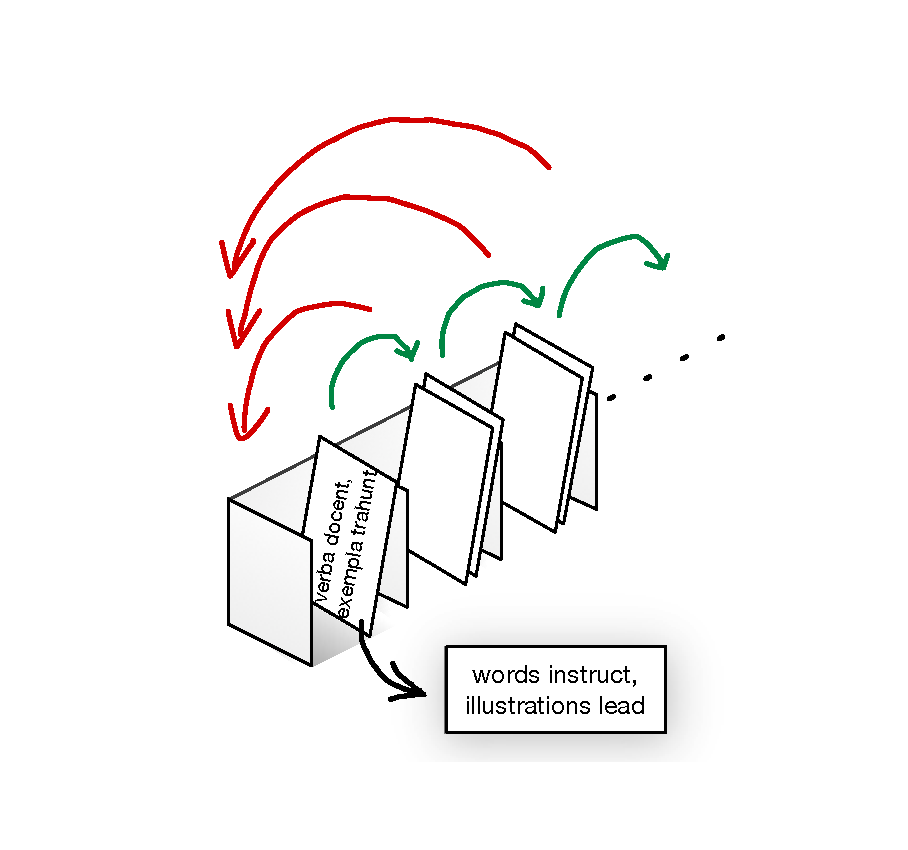
\includegraphics[width=0.4\textwidth]{membox_illustration.pdf}
	\caption{Static Structure of a Leitner's Learning Box}
	\label{fig:membox_depiction}
\end{figure}

For a more detailed overview of the box and our goals, we recommend you read the introduction to Part II. But for now, enough discussion!

\begin{itemize}

\item[$\blacktriangleright$] To get started in Eclipse, press the \texttt{new} button and navigate to ``Examples/eMoflon Handbook Examples/''
(Fig.~\ref{eclipse:downloadWizard}).

\begin{figure}[htbp]
	\centering
  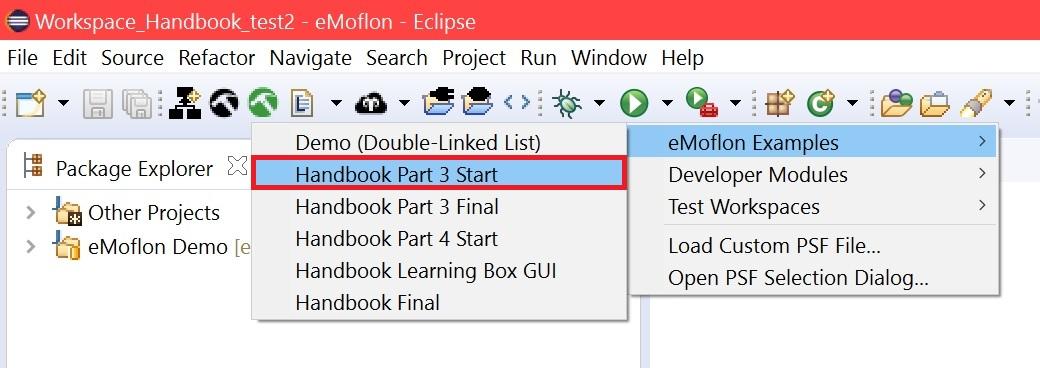
\includegraphics[width=0.75\textwidth]{eclipse_downloadWizard}
	\caption{Choose a cheat package}
	\label{eclipse:downloadWizard}
\end{figure}

\item[$\blacktriangleright$] Choose the cheat package for Part III and the syntax you prefer (textual or visual). Refer to Section 1 from Part I for details on
the differences between our syntaxes. The cheat package contains all files created up to the example in this point, as well as a small GUI that will enable
you to experiment with your metamodel.

\newpage

\vspace*{0.5cm}

\item[$\blacktriangleright$] If your package explorer does not resemble ours in Fig.~\ref{eclipse:workingSets} with at least two distinct nodes, select the
small, downward facing arrow in the corner of the package explorer. Choose ``Working Sets'' as your ``Top Level Elements.'' We use these to structure the
workspace in Eclipse.

\vspace{0.75cm}

\end{itemize}

\begin{figure}[htbp]
	\centering
  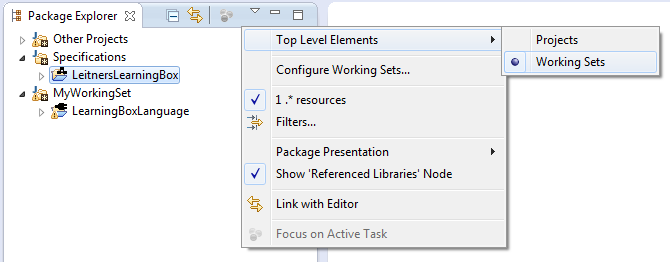
\includegraphics[width=0.9\textwidth]{eclipse_workingSets}
	\caption{Configuring your Package Explorer}
	\label{eclipse:workingSets}
\end{figure}

The ``MyWorkingSet" node contains \texttt{Learn\-ing\-Box\-Lang\-uage}, which in turn contains all the code generated from your metamodel. The metamodel itself
is found in \texttt{Leit\-ners\-Learn\-ing\-Box} under ``Specifications.'' The visual metamodel is a single \texttt{.eap} file, while the textual metamodel is
contained within an explicit folder structure, starting with ``/MOSL.'' Finally, the GUI is placed in the ``Other Projects'' node.

Each of these projects are not placed in the same working set as they have different \emph{nature}s, or project types. \texttt{Learning\-Box\-Language} is a
\emph{repository project}, the Eclipse classification of a normal Java project,\footnote{For details on the project setup, review Part I, Section 4}
while \texttt{LeitnersLearningBox} is a metamodel project.

\begin{itemize}

\item[$\blacktriangleright$] Inspect the files in both projects until you feel comfortable with what you'll be working with. In particular, look at the files
found under ``gen." Each Java file has a corresponding \texttt{.impl} file, where all generated method implementations will be placed.\footnote{For
more details on code generation, refer to Part I, Section 5} 

\item[$\blacktriangleright$] Be sure to also review the Ecore model in ``LearningBoxLanguage/model/'' and the dynamic model found in ``instances.'' While
you can make and customize your own instances,\footnote{To learn how to make your own instance models, review Part II, Section 4} we have included a small
sample to help you get started.

\end{itemize}

Well, that's it! A quick review, paired with a fine cheat package makes an excellent appetizer to SDMs. Let's get started.